% UC Davis poster built from the Gemini theme
% (https://github.com/anishathalye/gemini) and inspired by
% Rylan Schaeffer's Stanford template
% (https://github.com/RylanSchaeffer/Stanford-LaTeX-Poster-Template).
%
% COMPILE WITH XeLaTeX (Overleaf: Menu > Settings > Compiler > XeLaTeX).
% The Gemini theme uses fontspec, which requires XeLaTeX or LuaLaTeX.

\documentclass[final]{beamer}

% ====================
% Packages
% ====================

\usepackage[T1]{fontenc}
\usepackage{lmodern}
\usepackage[size=custom,width=120,height=72,scale=1.0]{beamerposter}
\usetheme{gemini}

% Force the Title to be Bold
\setbeamerfont{title}{series=\bfseries}

\usecolortheme{ucdavis}
\usepackage{graphicx}
\usepackage{booktabs}
\usepackage{tikz}
\usepackage{pgfplots}
\usepackage[most]{tcolorbox}
\pgfplotsset{compat=1.17}

% ====================
% Lengths — RECALCULATED FOR 3 EQUAL COLUMNS
% ====================

\newlength{\sepwidth}
\newlength{\colwidth}
\setlength{\sepwidth}{0.025\paperwidth}
\setlength{\colwidth}{0.30\paperwidth}

\newcommand{\separatorcolumn}{\begin{column}{\sepwidth}\end{column}}

% ====================
% Title / authors
% ====================

\title{Risk Estimation of Preeclampsia}

\author{\LARGE Ahmed Khan \and Lawrencedel Legaspi \and Selena Phu}

\institute[shortinst]{%
  \large
  \centerline{\textbf{Faculty Advisors:} Dr.\ Lihong Mo, MD, PhD (OB/GYN, UCDH) \textbullet\ Dr.\ Chen-Nee Chuah, PhD (ECE, UCD)}
  \vspace{0.3em}
  \centerline{\textbf{Graduate Mentors:} Hana Shaik, Arielle Yoo}
}

% ====================
% Footer
% ====================

\footercontent{%
  \rlap{\href{https://github.com/AhmedKhan-GH/repnet}{github.com/AhmedKhan-GH/repnet}}%
  \hfill
  UC Davis Senior Design Showcase 2026%
  \hfill
  \llap{\href{mailto:aekhan@ucdavis.edu}{aekhan@ucdavis.edu} | \href{mailto:lawlegaspi@ucdavis.edu}{lawlegaspi@ucdavis.edu} | \href{mailto:slphu@ucdavis.edu}{slphu@ucdavis.edu}}}

% ====================
% Logos & Typography Panel
% ====================

% Adjusted horizontal spacing to perfectly center the QR code inside the open visual gap
\logoleft{%
  \makebox[0pt][l]{%
    \ensuremath{\vcenter{\hbox{
\includegraphics[height=9cm]{logo.png}}}}% Left RUbiNet Logo
    \hspace*{5.8cm}% Fine-tuned spacing to position the QR code exactly in the middle of the gap
    \ensuremath{\vcenter{\hbox{
\includegraphics[height=8.0cm]{qrcode.png}}}}% Correct size-profile QR code
  }%
}

% Standard right logo placement evenly spaced
\logoright{%
  \setlength{\tabcolsep}{0pt}%
  \begin{tabular*}{\colwidth}{@{\extracolsep{\fill}} c c c}
    & \ensuremath{\vcenter{\hbox{\hspace*{1cm}
\includegraphics[height=5.5cm]{ece_header_white_text.png}}}} & \ensuremath{\vcenter{\hbox{\color{white}\fontsize{80}{80}\selectfont\bfseries 117}}}
  \end{tabular*}%
}

% ====================
% Body
% ====================

\begin{document}

\begin{frame}[t]

\begin{columns}[t]
\separatorcolumn

% =========================================================
% Column 1 — Background, Data, & Neural Network Introduction
% =========================================================
\begin{column}{\colwidth}

  \begin{block}{Introduction}
    Preeclampsia is a hypertensive disorder of pregnancy that can occur after 20 weeks of gestation~\cite{mayoclinic_preeclampsia}. Butler et al.\ showed a ResNet CNN can detect preeclampsia from raw ECG waveforms~\cite{butler2024preeclampsia}. We present RepNet, a pair of machine-learning models for risk estimation of preeclampsia from 12-lead ECGs. RepNet-SE is a channel independent convolutional neural network and RepNet-RF is a decision-tree ensemble trained on features extracted via NeuroKit2 and GE MUSE-reported measurements. We used 2,178 clinical 12-lead ECGs (335 PreE+, 15.4\%) from 1,383 patients at UC Davis Health.
  \end{block}

  \begin{block}{RepNet-SE: Neural Network Methods}
    RepNet-SE is a per-lead CNN: each of the 12 leads passes independently through a shared-weight 3-stage 1D convolutional backbone (kernels 31/21/11, Mish activations, strided downsampling). The pooled per-lead features are concatenated into a 576-dim vector and mapped to logits by a single linear layer (29,490 parameters).

    \begin{itemize}
      \item \textbf{Preprocessing:} Per-lead 0.5\,Hz high-pass (baseline wander removal), 60\,Hz notch filtering, z-score normalization, and downsampling to 250\,Hz
      \item \textbf{Training:} AdamW with cosine annealing and focal loss ($\gamma=1.0$) over a class-balanced sampler, early stopping on validation AUROC; evaluated across 30 patient-grouped 80/20 splits (no patient leakage)
    \end{itemize}
  \end{block}

  \begin{block}{RepNet-SE: Neural Network Results}
    \begin{figure}
      \centering
      % ONLY THESE TWO PLOTS ARE SHRUNK TO PREVENT BOTTOM OVERFLOW
      
\includegraphics[width=0.82\colwidth]{roc_pr_curves.png}
    \end{figure}
    \vspace{-1.5em}
    \begin{figure}
      \centering
      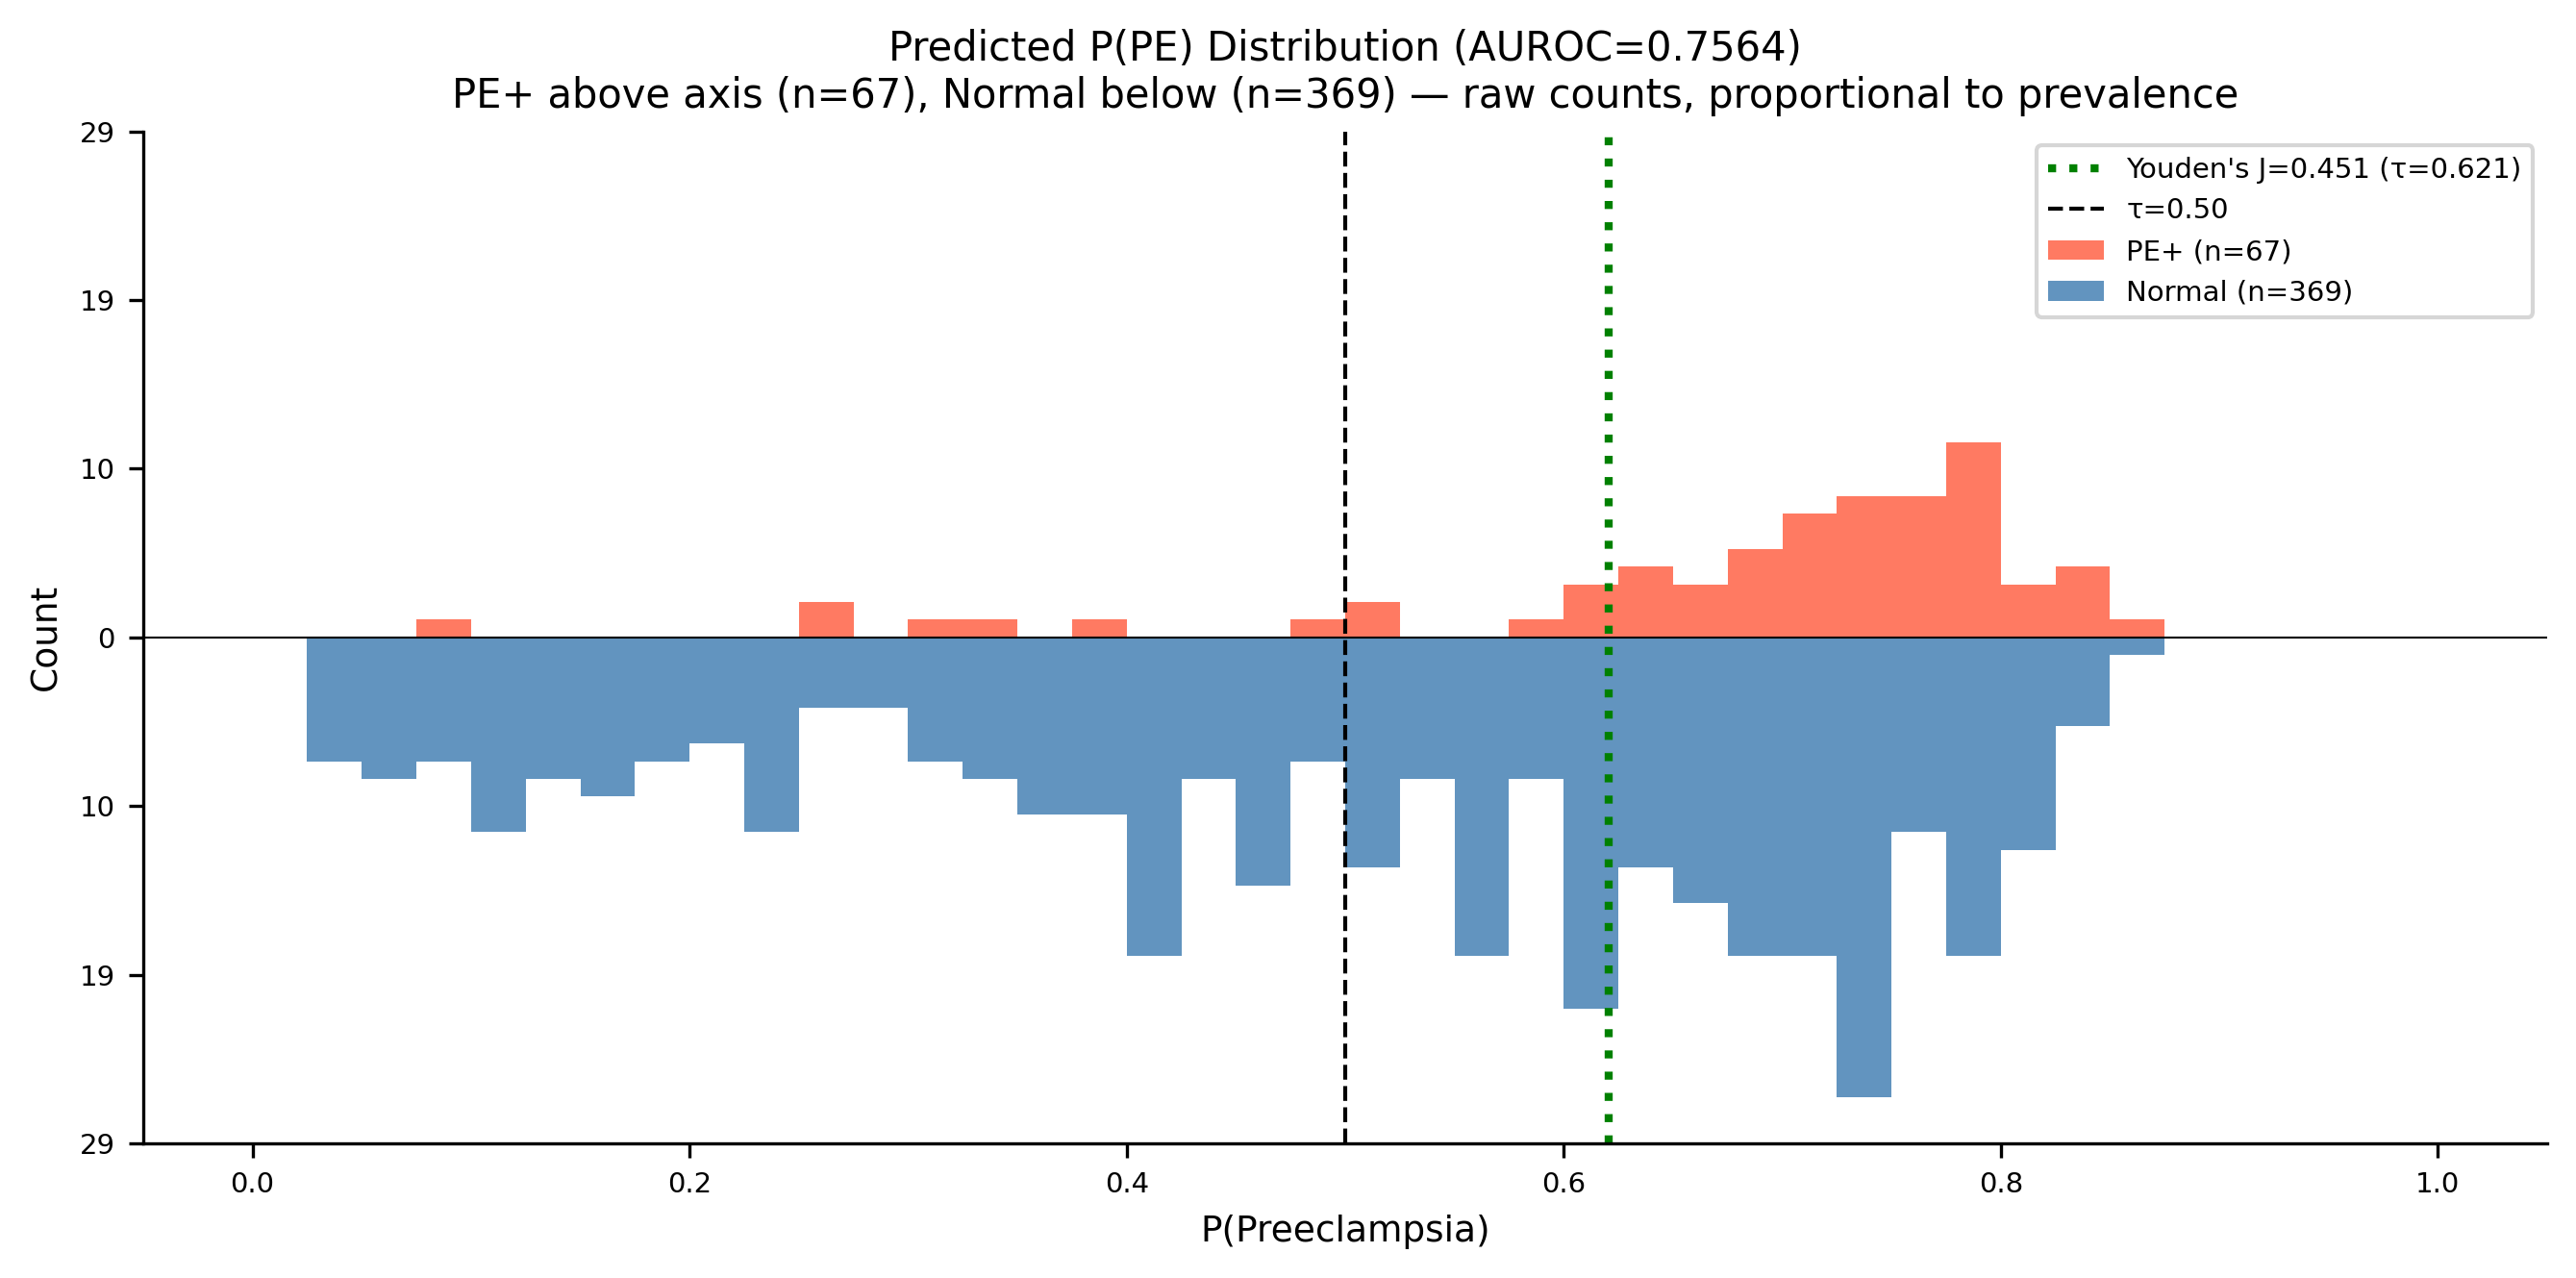
\includegraphics[width=0.86\colwidth]{pred_histogram.png}
    \end{figure}
    \vspace{-0.5em}

    Best split: AUROC = 0.779, AUPRC = 0.485 (test $n=446$, 15.7\% PE+). The model separates classes well (Youden's J = 0.439), though raw scores are skewed high (Brier = 0.483) with an optimal threshold at $\tau = 0.915$.
  \end{block}

\end{column}

\separatorcolumn

% =========================================================
% Column 2 — Deep Interpretability Dashboard
% =========================================================
\begin{column}{\colwidth}

  \vspace{2.4cm}

  \begin{table}
    \centering
    \footnotesize
    \resizebox{0.95\colwidth}{!}{%
    \begin{tabular}{l c c c c c c}
      \toprule
      \textbf{Operating Point} & \textbf{AUROC} & \textbf{AUPRC} & \textbf{Spec.} & \textbf{Sens.} & \textbf{Bal.\ Acc.} & \textbf{F1} \\
      \midrule
      Youden's J ($\tau\!=\!0.61$) & 70.9$\pm$4.9 & 34.2$\pm$7.5 & 62.7$\pm$12.6 & 73.0$\pm$9.2 & 67.9$\pm$3.8 & 40.4$\pm$6.9 \\
      Sens.\ $\geq$ 80\% ($\tau\!=\!0.55$) & 70.9$\pm$4.9 & 34.2$\pm$7.5 & 49.6$\pm$8.9 & \textbf{80.7$\pm$0.5} & 65.1$\pm$4.4 & 36.7$\pm$6.1 \\
      \bottomrule
    \end{tabular}%
    }
  \end{table}
  \vspace{0.5em}
  {\small Mean $\pm$ std over 30 patient-grouped 80/20 splits (29{,}490 params).\par}

  \begin{block}{RepNet-SE: Model Interpretability}
    \begin{figure}
      \centering
      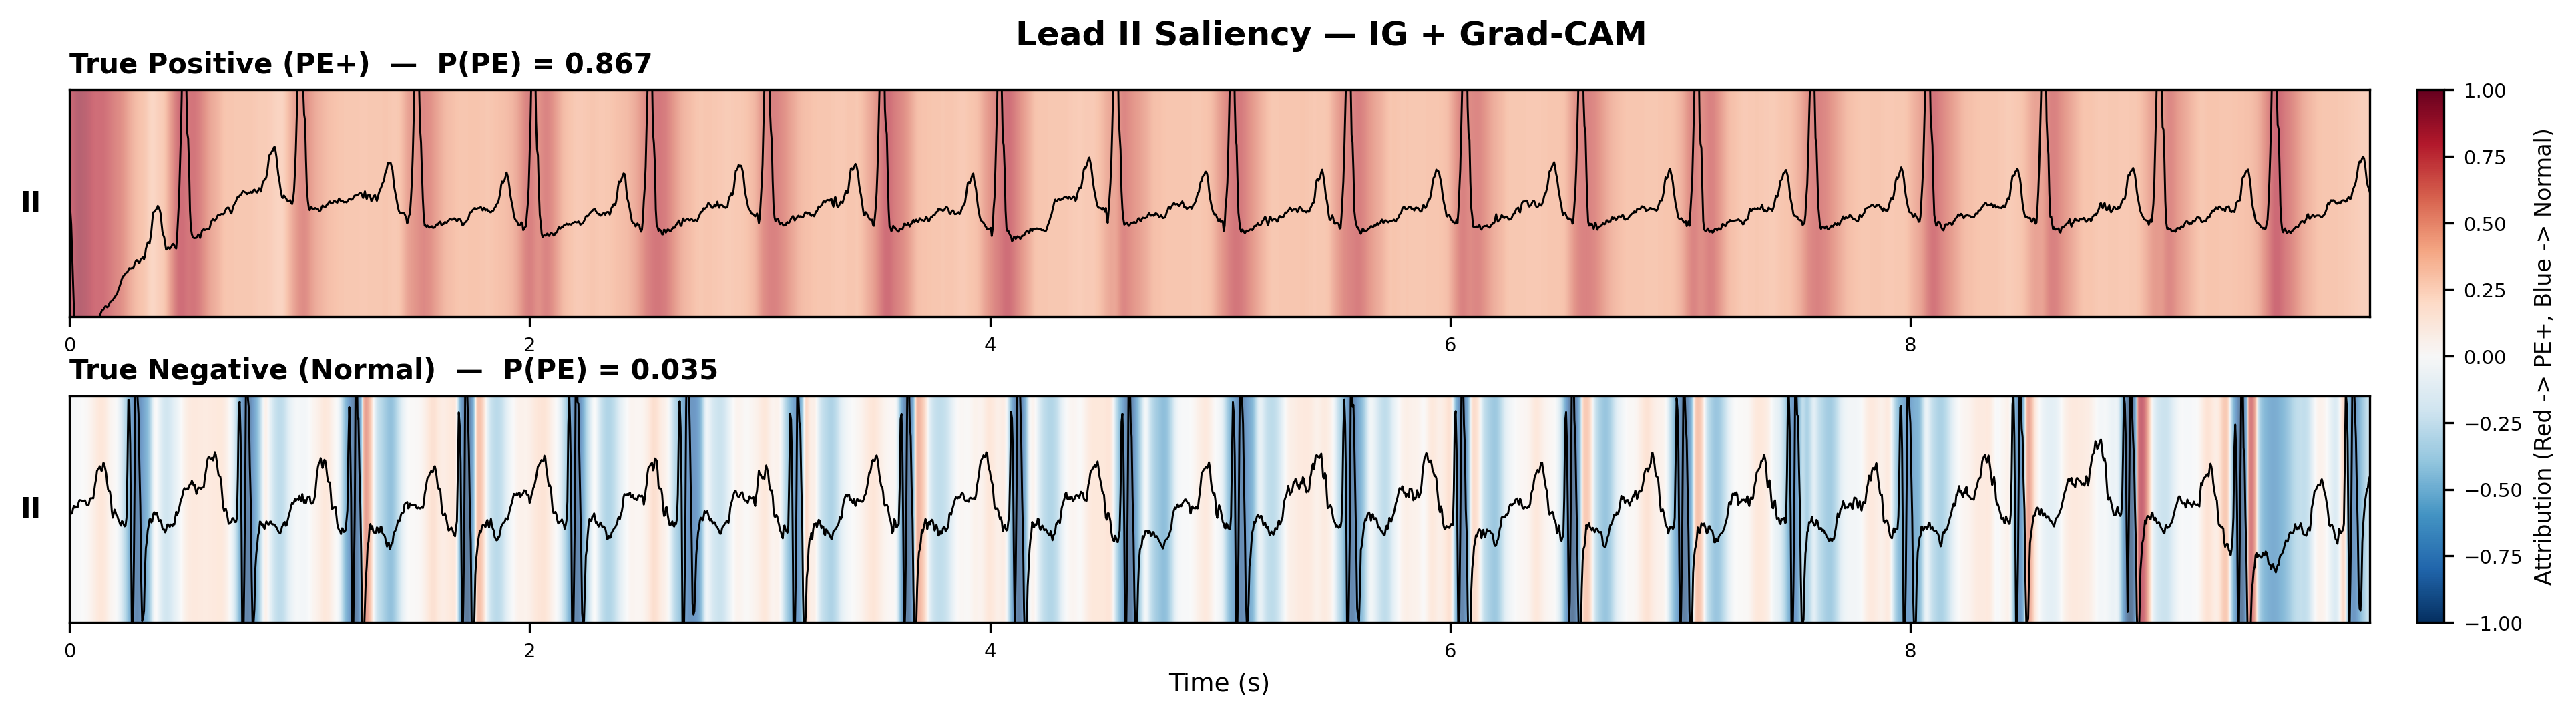
\includegraphics[width=\colwidth]{saliency_poster_lead_II.png}
    \end{figure}

    Combined Integrated-Gradients and Grad-CAM saliency on Lead II concentrates on the QRS complexes and ST segments. True positives attribute toward PE (red); true negatives attribute toward Normal (blue) at the same complexes.
  \end{block}

  \begin{block}{RepNet-RF: Decision-Tree Methods}
    \begin{itemize}
      \item Use NeuroKit2 to extract features from ECG data and combine with MUSE-reported features
      \item Feature importance analysis: Pearson Correlation, ANOVA, RFE (scoring on balanced accuracy, AUROC, and average precision)
      \item Train Random Forest model and with 5-fold StratifiedGroupKFold and RandomUnderSampler
      \item Train and evaluate ensemble methods
    \end{itemize}
    Ensembles evaluated were unweighted/weighted voting, stacking, and bagging. When choosing weights for weighted voting, it was important to assigner higher weights to the individually tuned models that performed better in terms of AUPRC and sensitivity.

    \vspace{-0.2em}
    % Native High-Performance Table Code containing the fixed formula configuration
    \begin{table}
  \centering
  \normalsize
  \setlength{\tabcolsep}{6pt}
  \renewcommand{\arraystretch}{1.3}
  \begin{tabular*}{\colwidth}{@{\extracolsep{\fill}} l l | l l}
    \toprule
    \textbf{Feature} & \textbf{Equation} & \textbf{Feature} & \textbf{Equation} \\
    \midrule
    $P_{\max}$ & {\small $\max_{\ell}(P_{\text{off}}^{\ell} - P_{\text{on}}^{\ell})$} & $T_{pe}/\text{QT}$ & {\small $T_{pe} / (T_{\text{off}} - R_{\text{on}})$} \\
    $P_{\min}$ & {\small $\min_{\ell}(P_{\text{off}}^{\ell} - P_{\text{on}}^{\ell})$} & $T_{pe}/\text{QTc}$ & {\small $(T_{pe} / \text{QT}) \cdot \sqrt{\Delta R_{pk}}$} \\
    P-Wave Disp. & {\small $P_{\max} - P_{\min}$} & ST Elev./Dep. & {\small $\mathbf{1}[>50\%\ \text{ST shift}]$} \\
    QT Disp. & {\small $\text{QT}_{\max} - \text{QT}_{\min}$} & Amp. Diff. & {\small $A_{\text{ST}} - A_{\text{PR}}$} \\
    $T_{pe}$ & {\small $(T_{\text{off}} - T_{\text{pk}})$} & QRS-T Angle & {\small $|\text{QRS Ax.} - \text{T Ax.}|$} \\
    QRS Axis & {\small $\perp\,\arg\min_{\ell}|\Sigma\,\text{QRS}^{\ell}|$} & T Axis & {\small $\perp\,\arg\min_{\ell}|\Sigma\,\text{T}^{\ell}|$} \\
    \bottomrule
  \end{tabular*}
\end{table}
    \vspace{-0.2em}
    {\footnotesize Per-lead features ($T_{pe}$, $T_{pe}$/QT, $T_{pe}$/QTc, ST elev./dep.) are computed for all 12 leads.\par}
    \vspace{-0.5em}
  \end{block}

\end{column}

\separatorcolumn

% =========================================================
% Column 3 — Decision-Tree Metrics, Outcomes, & Closings
% =========================================================
\begin{column}{\colwidth}

  \begin{block}{RepNet-RF: Decision-Tree Results}
    Unweighted Voting with SVM and LogisticRegression proved to be the best model when focusing on sensitivity/balanced accuracy. We look at these metrics to understand how well the model is correctly identifying preeclamptic ECGs and whether or not the model is genuinely distinguishing correctly between a normal or preeclamptic ECG.

    \begin{table}
      \centering
      \footnotesize
      \resizebox{0.95\colwidth}{!}{%
      \begin{tabular}{l c c c c c c}
        \toprule
        \textbf{Ensemble} & \textbf{AUROC} & \textbf{AUPRC} & \textbf{Spec.} & \textbf{Sens.} & \textbf{Bal.\ Acc.} & \textbf{F1} \\
        \midrule
        Unweighted Voting & 74.54$\pm$4.16 & 41.81$\pm$7.86 & 74.26$\pm$3.95 & 59.32$\pm$10.70 & 66.79$\pm$3.60 & 38.94$\pm$2.99 \\
        Weighted Voting & {74.75$\pm$4.35} & 42.26$\pm$7.92 & \textbf{74.75$\pm$4.48} & 60.23$\pm$10.88 & 67.49$\pm$3.45 & 39.80$\pm$2.76 \\
        \textbf{Unwtd.\ + SVM/LR} & \textbf{75.72$\pm$3.94} & 41.58$\pm$8.03 & 74.64$\pm$ 4.70 & \textbf{62.35$\pm$10.93} & \textbf{68.50$\pm$3.22} & \textbf{40.85}$\pm$2.24 \\
        Stacking & 74.77$\pm$4.35 & \textbf{42.43$\pm$7.59} & 74.37$\pm$4.18 & 59.62$\pm$10.80 & 67.00$\pm$3.46 & 39.17$\pm$2.79 \\
        Bagging CatBoost & 74.81$\pm$4.98 & 41.96$\pm$8.86 & 74.70$\pm$4.68 & 59.62$\pm$15.19 & 67.16$\pm$5.59 & 39.10$\pm$5.21\\
        \bottomrule
      \end{tabular}%
      }
    \end{table}
    
    \begin{figure}
      \centering
      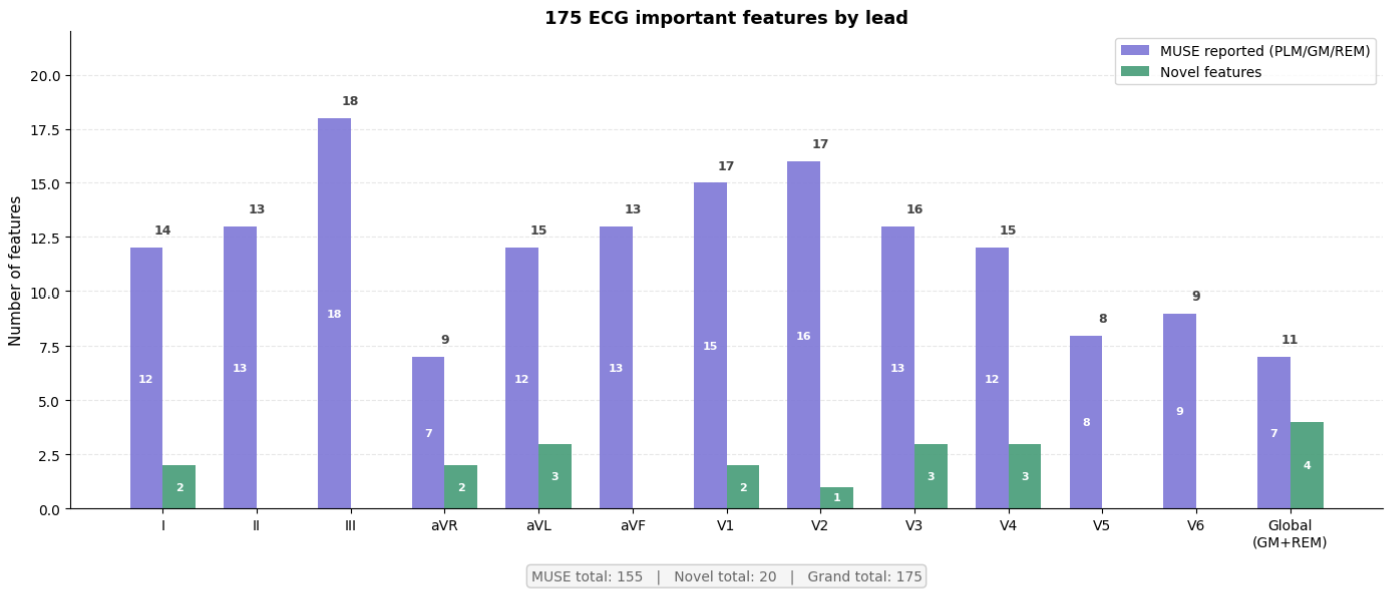
\includegraphics[width=0.86\colwidth]{leadimportance.png}
    \end{figure}
  \end{block}

  \begin{block}{Conclusion}
    RepNet-SE achieves a mean AUROC of 0.709 and RepNet-RF a mean AUROC of 0.757 in patient-grouped cross-validation, demonstrating that 12-lead ECGs contain discriminative signal for preeclampsia risk estimation despite 5.5:1 class imbalance. Both models independently converge on clinically relevant markers --- QRS morphology, ST-segment changes, $\mathnormal{T_{pe}}$ interval --- consistent with known cardiac effects of preeclampsia. Integrated-Gradients and Grad-CAM saliency confirm the neural network learns these patterns without explicit feature engineering. Broad ECG-based screening can enable early risk estimation and improve maternal and fetal outcomes.
  \end{block}

  \begin{block}{Future Work}
    \begin{itemize}
      \item \textbf{Lead Reduction \& Wearables:} Reduced lead sets (e.g. leads I, II, V2, V4) or single-lead models could enable screening via smart wearables such as Apple Watch ECGs
      \item \textbf{Transfer Learning:} Pretraining on large public ECG corpora (PTB-XL, MIMIC-IV-ECG) or leveraging ECG foundation models before fine-tuning on the UCDH cohort.
      \item \textbf{Multi-Site Validation:} Current results are from a single site; external validation on diverse populations is needed to assess generalizability.
      \item \textbf{Demographic Integration:} Incorporating maternal age, gestational age, and clinical history as auxiliary inputs alongside ECG data.
    \end{itemize}
  \end{block}

\end{column}

\separatorcolumn
\end{columns}
\end{frame}

\end{document}